\documentclass[conference]{IEEEtran}
% \IEEEoverridecommandlockouts
% The preceding line is only needed to identify funding in the first footnote. If that is unneeded, please comment it out.
\usepackage{cite}
\usepackage{amsmath,amssymb,amsfonts}
\usepackage{algorithmic}
\usepackage{graphicx}
\usepackage{textcomp}
\usepackage{xcolor}
\usepackage{hyperref}
\def\BibTeX{{\rm B\kern-.05em{\sc i\kern-.025em b}\kern-.08em
    T\kern-.1667em\lower.7ex\hbox{E}\kern-.125emX}}
\begin{document}

\title{Course Allocation System}


\author{\IEEEauthorblockN{Lokesh Venkatachalam}
\IEEEauthorblockA{\textit{Undergraduate Researcher} \\
\textit{Center for Security, Theory, Algorithms and Research (CSTAR)} \\
\textit{International Institute of Information Technology - Hyderabad}\\
Hyderabad, India \\
lokesh.v@research.iiit.ac.in}
}

\maketitle

\begin{abstract}
Course allocation the problem of allocating seats in university courses 
satisfying the upper bound of number of students, 
the credits of the student in a given semester in manner.
such that maximum numbers of students get the courses they have preferenced.\\
This paper proposes a novel software System to course allocation 
where students can make informed decisions about the course preferences,
administration and faculty can allocate the courses such that maximum number of students are happy.\\
\end{abstract}

\section{ \textbf{Introduction}} 
Course allocation has two major components, students giving the preferences and faculty,administration allocating the courses.\\
Students usually gather information from seniors about course content, gradings,professor etc
But the information about previous allocation is not well known among students, 
which makes it tougher for them to make informed decisions.\\
So in the proposed software system there will information about 
\begin{itemize}
\item Proposed course content, grading policy.   
\item Earlier course content, grading policy if exists
\item Earlier course allocation, students preference data
\end{itemize}

Many courses in university have a upper bound on number of students who can take it.
Some courses might also have lower bound on number of students for the course to proceed.
Student have also have to satisfy the minimum number of credits for a semester.
In certain universities students are given option to give more than preference for a given course type,
but in other universities students are allowed to give only one preference for a given course type in a given round of allocation
In most cases universities use simple first come first serve (FCFS) is used to allocate courses, 
which puts students without good internet, computer system at time of portal opening,etc on a disadvantage. 
It becomes like a lottery at the end. It also neither stable nor statergy proof.\\

So in this software system we are using the course allocation by stable matching algorithm \textbf{efficiency adjusted deferred acceptance mechanism (EADAM)}.
This algorithm is a modification of the  \textbf{Gale-Shapley student optimal stable mechanism (SOSM)} 
where the efficiency loss due to randomised tie-breaking is improved but at the expense of statergy-proofness[1].
This algorithm gives more no of students their higher order of their preferences.

\section{ \textbf{Literature Review} }

Allocation algorithms can be judges based on three major
parameters.
\begin{itemize}
\item \textbf{stability} - describes whether there exists a mapping where both students and teacher is betteer off
\item \textbf{strategy-proofness} - A algorithm is said to be statergy proof if the students
have no incentive to not give their true preference
\item \textbf{efficiency} - describes whether there can be another matching which is better to more students or faculty 
than one proposed by algorithnm at cost of few people. 
\end{itemize}
There is no existing algorithm which is STABLE, STATERGY PROOF and very efficient.
All algorithms have some drawback in atleast any one of the three parameters. 
\begin{itemize}
\item \textbf{First Come First Serve(FCFS)} is the most preffered algorithm, but is neither STABLE nor STATERGY PROOF. 
\item \textbf{Gale-Shapley student optimal stable mechanism (SOSM)} is STABLE and STATERGY PROOF, but more efficient algorithms exist[1].
\item \textbf{Efficiency Adjusted Deferred Acceptance mechanism(EADAM)} is STABLE and more efficient the SOSM but not statergy proof[1].
\end{itemize}

\section{ \textbf{System Architecture} }

In this section,I propose a software system for course allocation which will give basic information about each course 
to the students and an automatic course allocation based on students preferences reducing the manual work done by faculty and administration. 

\subsection{Users}

There are mainly there types of users.\\
\begin{itemize} 
\item \textbf{Administrators}\\
Users with highest level of access.
admin users job is add new students, faculty accounts to software system, 
update the course details,
update the credit requirements for students before each semester,
updating the time frame for course preferencing,
running the course allocation algorithm.

\item \textbf{Faculty}\\
Users with access to list the courses, give details about the courses, 
and have access to  previous data on student allocation.

\item \textbf{Student}\\
Students are the basic users who have the access to give one to three preferences to each course slot 
and also have access to view course content and previous allocation data
\end{itemize}
\subsection{Data}
\begin{enumerate}
\item Course Type 
    \begin{itemize}
    \item Name ex: Open elective, CS open elective , ECE open elective, Science , Math , Humanities, etc.
    \item credit: No of credits
    \end{itemize}
\item Course
    \begin{itemize}
    \item Course Type
    \item Course Code
    \item Course Name
    \item Course Description - Outline,Area,Prerequisites needed,recommended book, material etc
    \item Previous final course grading scheme
    \item Capacity
    \end{itemize}
\item Course Allocation Data contains:
    \begin{itemize}
    \item Course Name
    \item Year
    \item Semester
    \item Course Capacity of the year
    \item Faculty of the year
    \item No of students admitted as compulsory in round 1
    \item No of first preference in round 2
    \item No of second preference in round 2
    \item No of third preference in round 2
    \item No of first preference students allotted in round 2
    \item No of second preference students allotted in round 2
    \item No of third preference students allotted in round 2
    \item No of first preference in round 3
    \item No of second preference in round 3
    \item No of third preference in round 3
    \item No of first preference students allotted in round 3
    \item No of second preference students allotted in round 3
    \item No of third preference students allotted in round 3
    \item Faculty requests
    \item No of faculty requests accepted 
    \item total no of students who took the course at end.
    \item No of F grades.
    \item No of A grades.
    \end{itemize}
\item User
    \begin{itemize}
    \item User Email-ID
    \item User Type
    \end{itemize}
\end{enumerate}
\subsection{workflow}
\begin{itemize}
\item   
Credit requirements of students updated based on previous semester grades and students current semester requirements.
\item
Parallely faculty start to list the courses approved by dean/department head in course allocation software system with relevant details.\\
\item
After courses are listed, the lower bound (if exists) and upper bound on number students allowed to take the course are updated 
along with the previous years data of the course allocation for the courses listed.
\item Dates of choosing course preference are announced by administration after courses are listed.
\item First round of course allocation occurs where students are given the compulsory course they have to choose based on research/honours area.
\item The latest bound on course intake is updated after round one.
\item Round two starts, where students give three preferences for each course slot.
\item Round two allocation occurs. 
\item Students who were allotted there third preference are given a chance to choose or reject the course allocation.
\item Faculty taking a course can request the dean to allocate his course to few students who have not been allotted until end of round 2.
\item Round three starts, where students fill three preferences for each course slot which have not be allocated in round two.
\item Round three allocation occurs. 
\item Round four is manuall allocation to students who still have not been fulfill credit requirements after round three. 
\item With round 4 course allocation ends.
\end{itemize}
\begin{figure}[htbp]
    \centering
    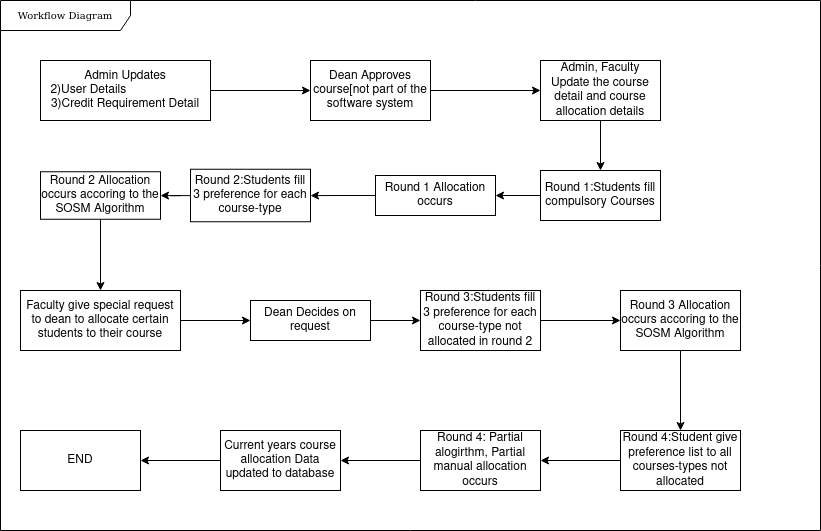
\includegraphics[width=\linewidth]{WF.png}
    \caption{Class UMl diagram \href{https://github.com/LokeshVenkatachalam/CODEFORCES/blob/main/Untitled2drawio.drawio.png}{Link}}
    \label{fig}
\end{figure}

\subsection{Use Cases}
\begin{figure}[htbp]
    \centering
    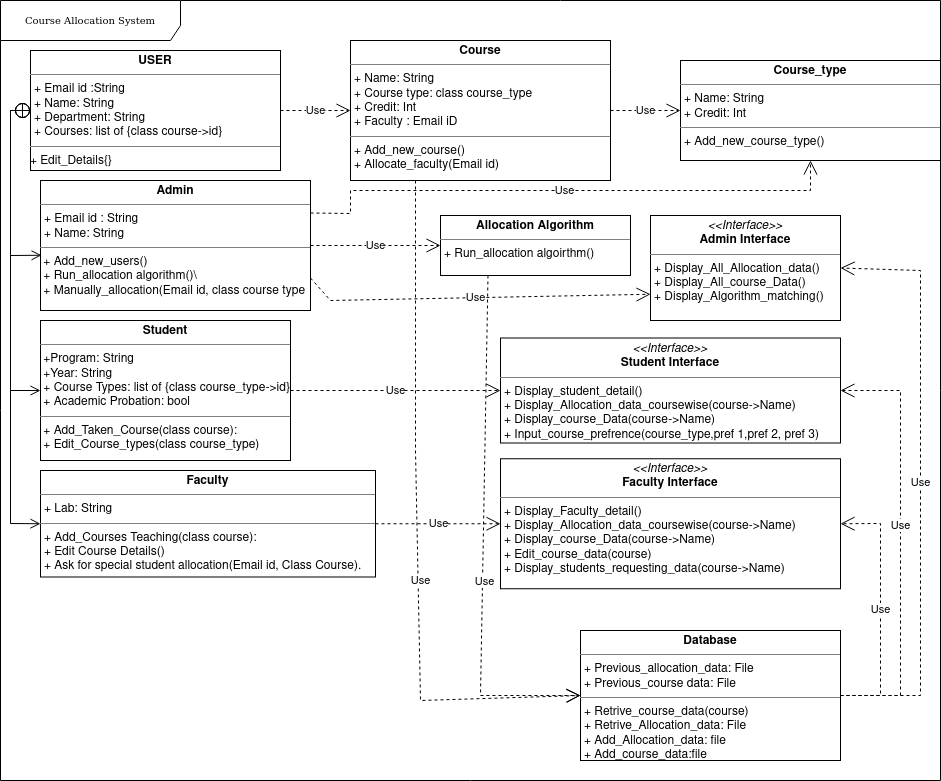
\includegraphics[width=\linewidth]{UML.png}
    \caption{Class UMl diagram \href{https://github.com/LokeshVenkatachalam/CODEFORCES/blob/main/x2.io.drawio.png}{Link}}
    \label{fig}
\end{figure}
\begin{enumerate}
    \item Authentication
        \begin{itemize}
        \item Admin creating new accounts with credentials.
        \item Student and Faculty logging in via CAS,
        \end{itemize}
    \item Data updating
        \begin{itemize}
        \item Admin updating course capacity
        \item Admin updating the previous years allocating data.
        \item Admin updating the credit requirements of the students. 
        \item Admin updating the time frame for course preferencing.
        \end{itemize}
    \item Course listing
        \begin{itemize}
        \item Admin/Professor listing the courses approved by dean/department head.
        \item Admin/Professor updating content of course information. 
        \end{itemize}
    \item Course preferencing 
        \begin{itemize}
        \item Students choose their course preference.
        \item Student ability to view the course information, previous allocation data.
        \end{itemize}
    \item Course Allocating 
        \begin{itemize}
        \item Admin runs the course allocation algorithm and allocates the course
        \item Admin/Professor can request the dean to allocate the courses to few students who have not been allotted until end of round 2.
        \end{itemize}
    \item Rounds
        \begin{itemize}
        \item The ability to run more than two rounds of allocation
        \end{itemize}
\end{enumerate}

\section{ \textbf{Conclusion and Future Work} }
The proposed software system makes it easier for administration to allocate courses and 
provides a more fairer chance in getting the wanted course.\\
We can options to give weightage to the preferenced courses, 
add option to see live course requesting data for students to see the demand.\\
Using the data collected from the allocation over period of years universities can work towards satisfying the demand each course gets.\\
The data can also be used for betterment of allocation algorithm.


\begin{thebibliography}{00}
\bibitem{b1} Franz Diebold, Haris Aziz, Martin Bichler, Florian
Matthes, and Alexander Schneider. Course Allocation
via Stable Matching. Business  Information Systems
Engineering, 6(2):97110, Apr 2014.

\end{thebibliography}
\vspace{12pt}
\end{document}
